\documentclass[
../../AuD-Zusammenfassung.tex,
]
{subfiles}

\externaldocument[ext:]{../../AuD-Zusammenfassung}
% Set Graphics Path, so pictures load correctly
\graphicspath{{../../}}

\begin{document}
\section{Laufzeitanalyse}
\subsection{O Notation}
Die O-Notation wird grundsätzlich für \textit{Worst-Case} Laufzeiten verwerdendet. Sie gibt also eine obere Schranke an, die der Algorithmus im schlechtesten Fall erreicht. Dabei wird oft zwischen Big O-Notation und Little o-Notation unterschieden. 
Ein Graph zur Repräsentation der O-Notation ist hier zu sehen:
\begin{center}
    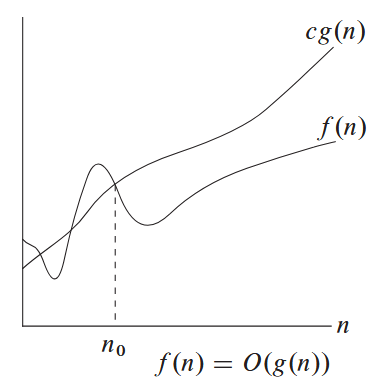
\includegraphics[scale=0.6]{Pics/ONotation.png}
\end{center}

\subsubsection{Big-O Notation}
Mathematische Definition: 
\begin{center}
    $O(g(n)) = \exists c \in \mathbb{R}_{>0}, n_0 \in \mathbb{N}, \forall n \geq n_0:  0 \leq f(n) \leq c \cdot g(n)$
\end{center}
Es existieren die positiven Konstanten $c$ und $n_0$ , sodass für alle $n \geq n_0$ gilt, dass  $f(n)$ $\geq$ 0 und $f(n)$ $\leq$ $c \cdot g(n)$. \\
Das bedeutet, dass die Funktion $f(n)$ für $n \to \infty$ den gleichen Wachstumsfaktor hat wie die Funktion $g(n)$.
Einfache Berechnung findet wie folgt statt (anhand vom Beispiel $f(n) = 5n^2 + 2n$):
\begin{enumerate}
    \item Finde den Term mit dem höchsten Wachstumsfaktor ($5n^2$)
    \item Konstanten werden weggelassen ($n^2$)
    \item Demnach ist $f(n) = O(n^2)$
\end{enumerate}
Dies kann man dann im Rückschluss so anwenden:
Um die Konstanten $c$ und $n_0$ zu finden, wird die obige gleichung benutzt:
\begin{enumerate}
    \item Simplifiziere die Ungleichung $5n^2 + 2n \leq c \cdot n^2$ zu $5 + \frac{2}{n} \leq c$
    \item Da $n \geq n_0$ kann man die Gleichung für $n \geq 1$ auflösen um die Konstanten $c$ und $n_0$ zu finden. \\
    $\implies$ $5 + \frac{2}{1} = 7 \leq c$ $\implies$ $c \geq 7$
    \item Dementsprechend kann man dann die Konstanten $c = 7$ und $n_0 = 1$ auswählen.
\end{enumerate}

\newpage
\subsubsection{Little-o Notation}
Mathematische Notation:
\begin{center}
    $O(g(n)) = \exists c \in \mathbb{R}_{>0}, n_0 \in \mathbb{N}, \forall n \geq n_0:  0 \leq f(n) < c \cdot g(n)$
\end{center}
Es existieren die positive Konstanten $c$ und $n_0$, sodass für alle $n \geq n_0$ gilt, dass  $f(n)$ $\geq$  0 und $f(n)$ $<$ $c \cdot g(n)$. Little-o Notation unterscheidet sich also von Big-O Notation nur oberen Schranke. Während bei Big-O der Wachstumsfaktor beider Funktion gleich sein kann ($f(n) = c \cdot g(n)$), gilt bei Little-o, dass der Wachstumsfaktor der Funktion $f(n)$ kleiner ist als der Wachstumsfaktor der Funktion $g(n)$. \\
Einfache Berechnung findet analog zu Big-O wie folgt statt (anhand vom Beispiel $f(n) = 5n^2 + 2n$):
\begin{enumerate}
    \item Finde den Term mit dem höchsten Wachstumsfaktor ($5n^2$)
    \item Konstanten werden weggelassen ($n^2$)
    \item Demnach ist $f(n) = o(n^2)$
\end{enumerate}
Hier muss allerdings noch geprüft werden, ob der Wachstumsfaktor der Funktion $f(n)$ kleiner ist als der Wachstumsfaktor der Funktion $g(n)$. Wenn ja, ist die Little-o Notation korrekt für $g(n)$. \\
Um zu zeigen, dass $f(n) = o(g(n))$:
\begin{enumerate}
    \item Finde den Limes des simplifizierten Ausdrucks $\frac{f(n)}{g(n)}$, der die Wachstumsrate der Funktion $f(n)$ zur Wachstumsrate der Funktion $g(n)$ vergleicht.
    \begin{itemize}
        \item $\lim_{n \to \infty} \frac{f(n)}{g(n)} = \lim_{n \to \infty} \frac{5n^2 + 2n}{n^2} = \lim_{n \to \infty} 5 + \frac{2}{n} = 5$\\
        $\impliedby \frac{2}{n}$ für $n \to \infty = 0$ 
    \end{itemize}
    \item Da der Limes $\not= 0$ ist, bedeutet das, dass der Wachstum von $f(n)$ nicht geringer ist als der von $g(n)$. Deshalb müssen wir ein Polynomgrad hochgehen, weswegen $f(n) = o(n^3)$ sein muss. 
    \item Um nun die Konstanten $c$ und $n_0$ zu finden müssen wir einfach $\frac{f(n)}{g(n)}$ auflösen
    \begin{itemize}
        \item $\frac{5n^2 + 2n}{n^3} < c$
        \item $\frac{5}{n} + \frac{2}{n^2} < c$
        \item $\frac{5}{n} < c$, da $\frac{2}{n^2}$ für $n \to \infty$ schneller abfällt als $\frac{5}{n}$
        \item Für $c = 1$ muss dann $n_0 > 5$ sein und kann somit als $n_0 = 6$ gewählt werden.
    \end{itemize}
\end{enumerate}

\subsubsection{Rechenregeln}
Die Rechenregeln für die O Notation sind:
\begin{itemize}
    \item Konstanten: $f(n) = a$ mit $a \in \mathbb{R}_{>0} \implies f(n) = O(1)$\\
    Ist die Funktion konstant so ist die Komplexität $O(1)$
    \item Skalare Multiplikation: $f(n) = O(g) \longrightarrow a \cdot f(n) = O(g)$\\ 
    Multiplikation der Funktion ändert Komplexität nicht.
    \item Addition: $f_1 = O(g_1), f_2 = O(g_2) \longrightarrow f_1 + f_2 = O(max\{g_1, g_2\})$\\
    Die Komplexität der Summe zweier Funktion ist der Maximalwert der Komplexität der beiden Funktionen.
    \item Multiplikation: $f_1 = O(g_1), f_2 = O(g_2) \longrightarrow   f_1 \cdot f_2 = O(g_1 \cdot g_2)$\\
    Die Komplexität des Produkts zweier Funktionen ist das Produkt der Komplexität der beiden Funktionen.
\end{itemize}

\newpage
\subsection{$\Omega$\space Notation}
Ähnlich zur O Notation, allerdings geht es hier um den \textit{Best-Case} also minimale Anzahl der Schritten, die ein Algorithmus ausführt.
\begin{center}
    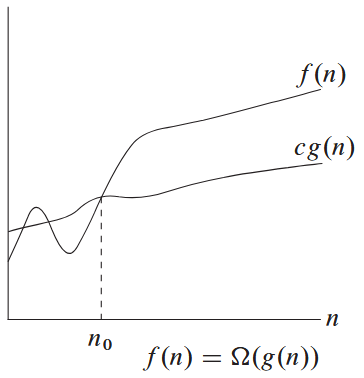
\includegraphics[scale=0.6]{Pics/OmegaNotation.png}
\end{center}
Wird auch wieder in $\Omega$ und $\omega$ aufgeteilt, die sich nur darin unterscheiden, wie strikt die Grenze ist.
\subsubsection{$\Omega$ Notation}
Mathematische Definition:
\begin{center}
    $\Omega(g(n)) = \exists c \in \mathbb{R}_{>0}, n_0 \in \mathbb{N}, \forall n \geq n_0:  0 \leq c \cdot g(n) \leq f(n)$
\end{center}
Es existieren die positiven Konstanten $c$ und $n_0$ , sodass für alle $n \geq n_0$ gilt, dass  $0 \leq c \cdot g(n) \leq f(n)$. 
Das bedeutet, dass der Wachstumsfaktor von $f(n) \geq c \cdot g(n)$ ist. \\

Die Berechnung von $\Omega$ ist leider nicht immer so simpel wie die Berechnung von O Notation. Nehme zum Beispiel einen Linearen Suchalgorithmus, der eine Liste so lange durchläuft, bis er die gesuchte Zahl gefunden hat. Die Komplexität ist $O(n)$, da, wenn das Element an letzter Stelle steht alle Eingaben durchlaufen werden müssen. Gleichermaßen kann es aber sein, dass das Element an erster Stelle steht, was dann die Komplexität $\Omega(1)$ besitzt. Dies muss allerdings durch Analyse des Algorithmus selbst erkannt werden und kann nicht aus der Funktionsrepräsentation ermittelt werden.\\
Gilt allerdings nicht sowas, wie vorzeitiger Abbruch bei Suche, so kann $\Omega$ ähnlich zu $O$ verwendet werden (Anhand vom Beispiel $f(n) = 5n^2 + 2n$):
\begin{enumerate}
    \item Finde den Term mit dem höchsten Wachstumsfaktor ($5n^2$)
    \item Konstanten werden weggelassen ($n^2$)
    \item Demnach ist $f(n) = \Omega(n^2)$\\
    Da $5n^2 + 2n$ für $n \to \infty$ mindestens so schnell wächst wie $n^2$.
\end{enumerate}
Um Werte für $c$ und $n_0$ zu finden, kann das Prinzip wie in O Notation verwendet werden, jedoch auf der Definition von $\Omega$ angepasst (Umgekehrtes Gleichheitsszeichen).
\newpage
\subsubsection{$\omega$ Notation}
Mathematische Definition:
\begin{center}
    $\omega(g(n)) = \exists c \in \mathbb{R}_{>0}, n_0 \in \mathbb{N}, \forall n \geq n_0:  0 \leq c \cdot g(n) < f(n)$
\end{center}
Es existieren die positiven Konstanten $c$ und $n_0$ , sodass für alle $n \geq n_0$ gilt, dass  $0 \leq c \cdot g(n) < f(n)$. \\
Das bedeutet, dass der Wachstumsfaktor von $f(n) > c \cdot g(n)$ ist. \\

Für die Bestimmung von $\omega$ gilt das selbe wie für $\Omega$, nur das zusätzlich noch folgendes beachtet werden muss: 
\begin{itemize}
    \item Hat der Algorithmus einen konstanten Best-Case, so ist $\omega$ nicht anwendbar, da $\omega < 1$ sinnlos ist, da per Definition die Komplexität nicht kleiner als 1 sein kann und so der Best-Case schon durch $\Omega$ definiert ist. 
    \item Falls nicht konstant, dann muss bei $\omega$ ähnlich zu Little-o herausgefunden werden, ob der Wachstumsfaktor von $f(n)$ strikt größer ist als der Wachstumsfaktor der Funktion $g(n)$.
    \begin{itemize}
        \item $\lim_{n \to \infty}\frac{f(n)}{g(n)}$
        \item Wenn $lim = \infty$, so gilt $\omega(g(n))$
        \item Andernfalls muss der Polynomgrad von $g(n)$ verringert werden:\\
        $\longrightarrow n^x = n^{x - 1} \implies n = 1$
    \end{itemize}
\end{itemize}

\subsubsection{Rechenregeln}
\newpage 
\subsection{$\Theta$\space Notation}

\begin{center}
    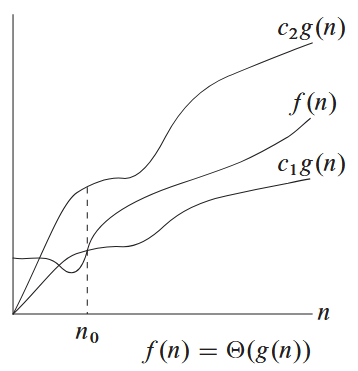
\includegraphics[scale=0.6]{Pics/LandauNotation.png}
\end{center}
\end{document}